\chapter{Métricas de Software}

\section{Processo de Medição de Software}

Segundo \citeonline{Fenton98}, medição é o mapeamento de relações empíricas em relações formais. Isto é, quantificação em símbolos com objetivo de caracterizar uma entidade por meio de seus atributos. Contrapondo-se com uma  definição operacional, a \citeonline{ISO:15939} define medição como conjunto de operações que visam por meio de um objeto determinar um valor a uma medida ou métrica \footnote{A definição formal da \citeonline{ISO:15939} não utiliza o termo métrica. Tendo em vista que o termo métrica é mais difundido em processos de medição e análise, tais os que se baseiam diretamente ou indiretamente no \textit{Goal-Question-Metric} de \citeonline{Basili96b}, resolveu-se adotar o termo métrica com mesmo valor semântico ao termo medida da \citeonline{ISO:15939}, que é o valor operacional propriamente dito}. Alguns modelos de referência, como \citeonline{cmmi2010}, e até a própria \citeonline{ISO:15939} definem medição como uma ferramenta primordial para gerenciar as atividades do desenvolvimento de software e para avaliar a qualidade dos produtos e a capacidade de processos organizacionais. 


A \citeonline{ISO:15939} define um processo de medição com base em um modelo de
informação, que é mostrado na Figura \ref{informação}, a fim de obter produtos de informação para cada necessidade de informação. Para isto, cada necessidade de informação, que é uma situação que requer conhecimento com intuito de  gerenciar objetivos, metas, riscos e problemas, é mapeada em uma construção  mensurável que tem em sua origem um conceito mensurável, como por exemplo,  tamanho, qualidade e custo a fim de mapear um atributo (característica  que permite distinguir qualitativamente e/ou quantitativamente) uma entidade que pode ser um processo, projeto ou produto de software. Por fim  cada construção mensurável é mapeada em um ou mais produtos de informação que  levam uma ou mais métricas ou medidas, que podem ser classificadas sob  critérios apresentados na Seção \ref{Classificação das Métricas de Software}.

\begin{figure}[h!]
\centering
	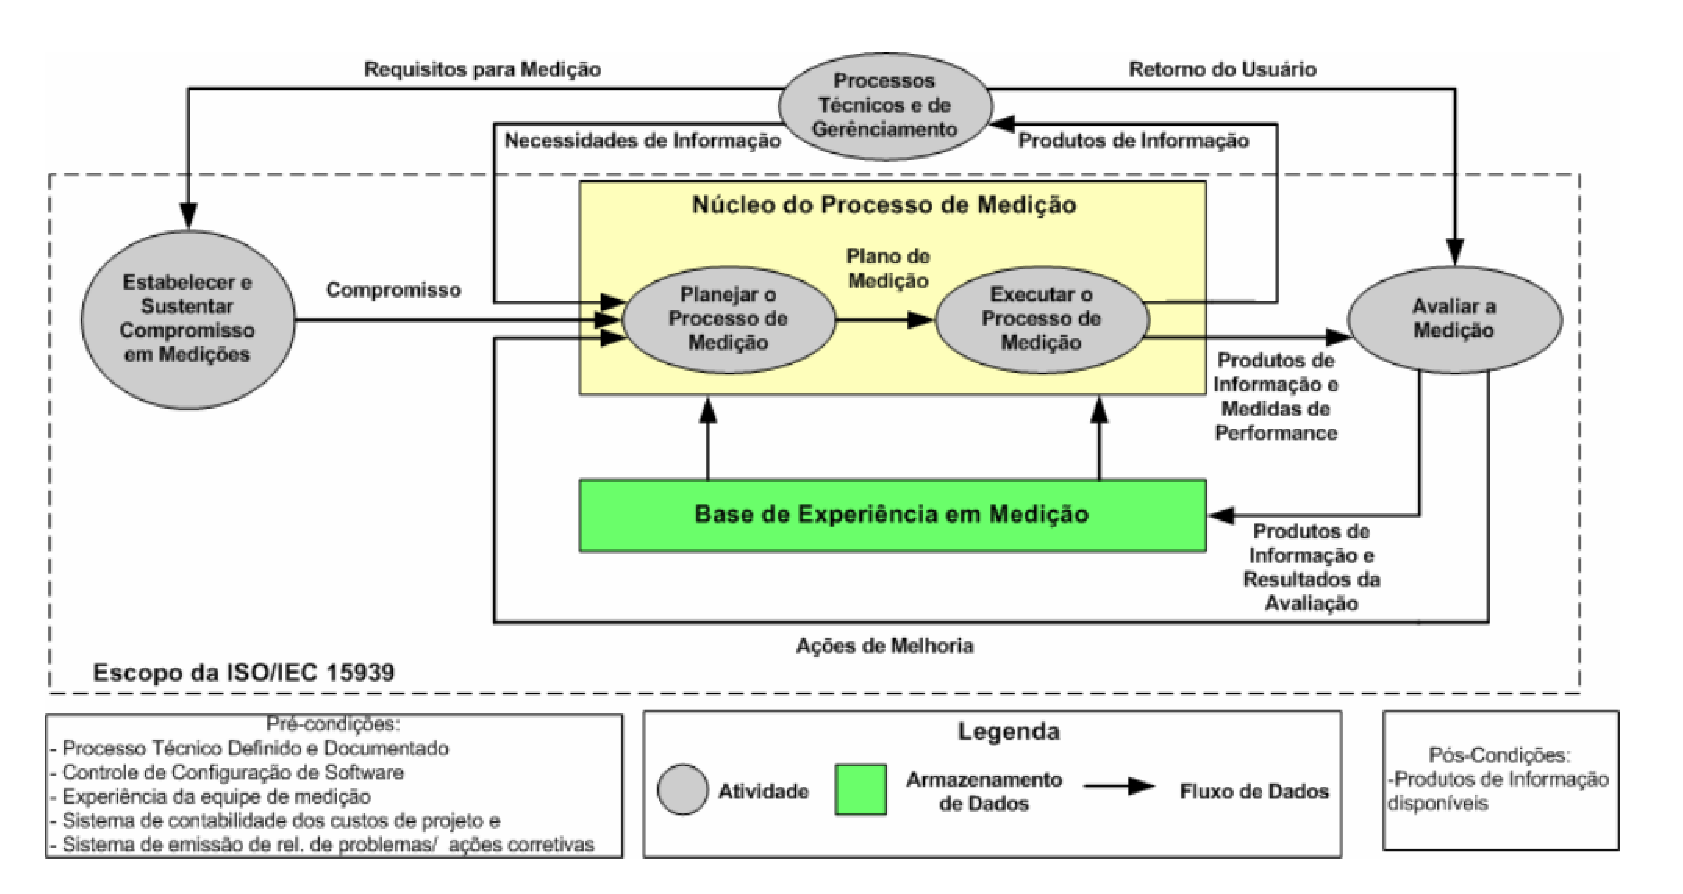
\includegraphics[keepaspectratio=true,scale=0.3]{figuras/processo15939.eps}
	\caption{Modelo de Informação da ISO 15939}
	\label{informação}
\end{figure}
\FloatBarrier

O modelo de informação da \citeonline{ISO:15939} é utilizado para construir o 
propósito geral da medições e a identificação de medidas ou métricas que 
respondem as necessidades de informação. Quando se trata da coletas de métricas de código-fonte, é possível construir um modelo de informação tal como na Tabela \ref{construção-código}.

	\begin{table}[!ht]
	\begin{center}
	
	\input{tabelas/modelo-informacao.ltx} 
	\caption{Modelo de Informação para métricas de código-fonte com base na 
	\citeonline{ISO:15939}}
	\label{construção-código}
	\end{center}
	\end{table}		

%---------------------------------------------------------------------------------------------------------------------%

\section{Classificação das Métricas de Software}	
\label{Classificação das Métricas de Software}

As métricas de software possuem uma escala de medição, que é um conjunto 
ordenado de valores, contínuos ou discretos, ou uma série de categorias nas 
quais entidade é mapeada \cite{ISO:15939}. As escalas podem ser:

\begin{easylist}[itemize]

& \textbf{Nominal:} A medição é categórica. Nesta escala, só é possível realização de comparações, sendo que a ordem não possui significado
\cite{ISO:15939} \cite{Fenton98} \cite{Meirelles2013}.

& \textbf{Ordinal:} A medição é baseada em ordenação, ou seja, os valores possuem 
ordem, mas a distância entre eles não possui significado. Por exemplo, nível 
de experiência dos programadores \cite{ISO:15939} \cite{Fenton98} 
\cite{Meirelles2013}. 

& \textbf{Intervalo:} A medição é baseada em distâncias iguais definidas para as 
menores unidades. Por exemplo, o aumento de 1º C de um termômetro. Nesta 
escala é possível realizar ordenação, soma e subtração
\cite{ISO:15939} \cite{Fenton98}. 

& \textbf{Racional:} A medição é baseada em distâncias iguais definidas para as 
menores unidades, e neste caso é possível a ausência por meio do zero 
absoluto. Por exemplo, a quantidade de linhas de código em uma classe. 
Nesta escala, é possível realizar ordenação, soma, subtração, 
multiplicação e divisão \cite{ISO:15939} \cite{Fenton98}. 

\end{easylist}
	
As métricas podem ser classificadas quanto ao objeto da métrica, que 
divide as métricas de software em: \textit{métricas de processo} e 
\textit{métricas de produto} \cite{Mills:1999}. Ainda é possível, segundo a 
\citeonline{ISO:15939}, dividir as métricas quanto ao método de medição, 
podendo estas serem \textit{métricas objetivas}, que são baseadas em regras 
númericas e podem ter a coleta manual ou automática, ou \textit{métricas 
subjetivas}, que envolvem o julgamento humano para consolidação do resultado. 

Segundo o modelo de qualidade da \citeonline{ISO25023}, que é mostrado na 
Figura \ref{modelodequalidade}, as métricas de produto podem ser subdivididas 
em três categorias: 

				
\begin{figure}[h!]
\centering
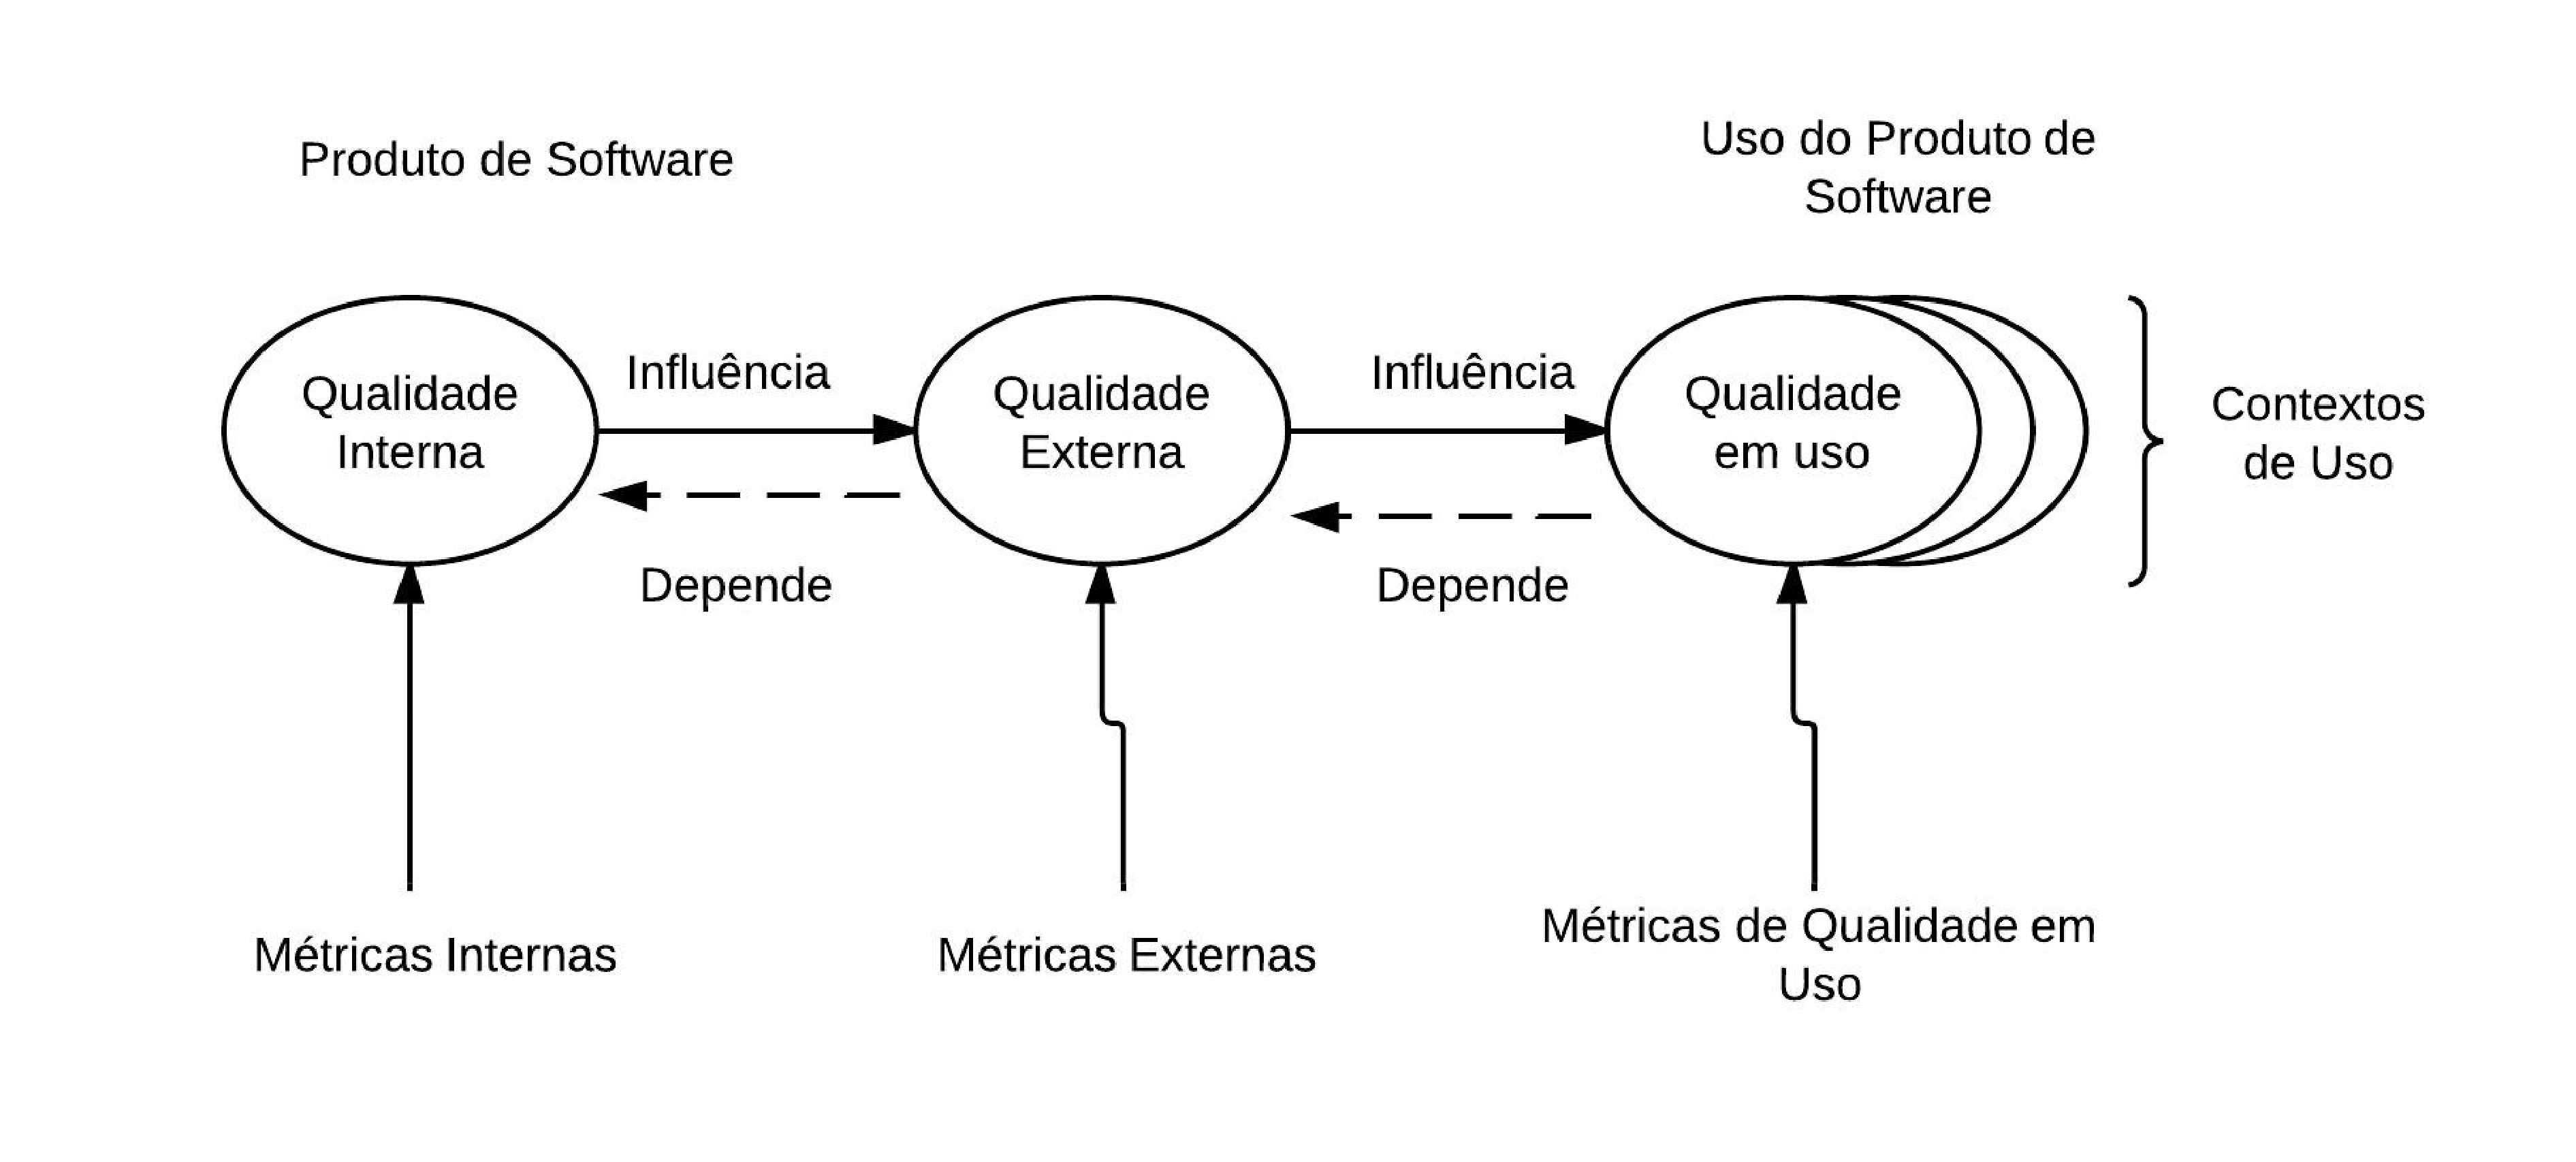
\includegraphics[keepaspectratio=false,scale=0.25]{figuras/modelodequalidade.eps}
\caption{Modelo de Qualidade do Produto da ISO 25023 adaptado da 
\citeonline{ISO25023}}
\label{modelodequalidade}
\end{figure}
\FloatBarrier

\begin{easylist}[itemize]
	
%-----------------------------
		& \textbf{Métricas Internas:} 
		São métricas que aferem a qualidade interna do software por meio da 
		avaliação de estruturas internas que compõem o software em estágio de 
		desenvolvimento. São conhecidas como métricas de código-fonte.

%-----------------------------			
		& \textbf{Métricas Externas:}
		São métricas que capturam o comportamento do software. Exemplos de 
		atributos da qualidade externa: correção, usabilidade, eficiência e 
		robustez. Qualidade externa mede o comportamento do software. Estas só 
		podem ser aferidas por atividades de teste do desenvolvimento do 
		software em condições similares as que serão encontradas em ambientes de
		implantação.

%-----------------------------			
		& \textbf{Métricas de Qualidade em Uso:}
		São métricas que aferem se o software atende as necessidades do cliente
		com eficiência, produtividade, segurança e satisfação em contextos 
		específicos de uso. Estas só podem ser coletadas em ambientes reais, 
		isto é, o ambiente de implantação.	
			 
\end{easylist}
		
				

%---------------------------------------------------------------------------------------------------------------------%
\section {Métricas de Código-Fonte}
\label{sec:source-code}

Segundo a \textit{International Working Conference on Source Code Analysis and 
Manipulation} (SCAM), o código-fonte é qualquer especificação executável 
de um sistema de software. Por conseguinte, se inclui desde código de máquina 
até linguagens de alto nível ou representações gráficas executáveis \cite{harman2010source}. Este fato significa que as métricas de código-fonte  são métricas objetivas e possuem características como validade, simplicidade, objetividade, fácil obtenção e robustez \cite{Mills:1999}. 


%--------------------------------------------
\subsection{Métrica de Tamanho e Complexidade}

\label{métricas tamanho e complexidade} 

O tamanho do código-fonte foi um dos primeiros conceitos mensuráveis do 
software, dado que o software poderia ocupar espaço tanto em forma de cartões 
perfurados quanto em forma de papel quando o código-fonte era impresso. 
A segunda lei de \citeonline{Lehman1980b} enuncia que a complexidade aumenta à 
medida que o software é evoluído. Logo, é perceptível que as métricas de complexidade 
estão diretamente ligadas as métricas de tamanho, sendo que a modificação em 
uma provavelmente impactará na outra. A seguir são apresentadas 
algumas métricas de tamanho e complexidade:

\begin{easylist}[itemize]


	& \textbf{LOC} (\textit{Lines of Code} - Número de Linhas de Código)
	foi uma das primeiras métricas utilizadas para medir o tamanho de um 
	software. São contadas apenas as linhas executáveis, ou seja, são excluídas linhas em branco e comentários. Para efetuar comparações entre sistemas usando LOC, é necessário que ambos tenham sido feitos na mesma linguagem de programação e que o estilo esteja normalizado \cite{Jones91}.
	
	& \textbf{ACCM} (\textit{Average Cyclomatic Complexity per Method} - 
	Média da Complexidade Ciclomática por Método) mede a complexidade dos 
	métodos ou funções de um programa. Essa métrica pode ser representada 
	através de um grafo de fluxo de controle \cite{McCabe76}. O uso de 
	estruturas de controle, tais como, \textit{if, else, while} aumentam a 
	complexidade ciclomática de um método.

	& \textbf{AMLOC} (\textit{Average Method Lines of Code} - Média do número de linhas de código por método)Essa medida indica se o código está bem distribuído entre os métodos. Quanto maior, mais pesados são os métodos. É preferível ter muitas operações pequenas e de fácil entendimento que poucas operações grandes e complexas \cite{Meirelles2013}.

\end{easylist}


\subsection{Métricas de Orientação à Objetos}
\label{métrica objetos}

A evolução dos paradigmas de programação permitiu que as linguagens de 
programação assumissem diversas características entre si. O
paradigma da orientação à objetos permitiu aos programadores abstrair computação ao negócio, isso significou evolução no desenvolvimento quando comparado ao paradigma procedural e permanência na academia quanto na indústria de desenvolvimento de sotware \cite{Li1993}.

Dado a grande utilização do paradigma no desenvolvimento de software, foram selecionadas algumas das principais métricas de orientação à objetos:


\begin{easylist}
	
	%--------------------------
	& \textbf{ACC} (\textit{Afferent Connections per Class} - Conexões Aferentes por Classe) é o número total de classes externas de um pacote que dependem de classes de dentro desse pacote. Quando 
	calculada no nível da classe, essa medida também é conhecida como 
	\textit{Fan-in} da classe, medindo o número de classes das quais a classe é derivada e, assim, valores elevados indicam uso excessivo de herança 
	múltipla \cite{McCabe94} \cite{Chidamber94}.

	%--------------------------
	& \textbf{ANPM} (\textit{Average Number of Parameters per Method} - Média do Número de Parâmetros por Método) alcula a média de parâmetros dos métodos da classe. Seu valor mínimo é zero e não existe um limite máximo para o seu resultado, mas um número alto de parâmetros pode indicar que um método pode ter mais uma responsabilidade \cite{Basili1987}


	%--------------------------
	& \textbf{CBO} (\textit{Coupling Between Objects} - Acoplamento entre Objetos) é o número total de classes dentro de um pacote que dependem de classes externas ao pacote. Quando calculada no nível da classe, essa medida também é conhecida como Fan-out da classe \cite{Chidamber94}


	%-----------------------------
	& \textbf{DIT} (\textit{Depth of Inheritance Tree} - Profundidade da 
	Árvore de Herança) é o número de superclasses ou classes ancestrais da 
	classe sendo analisada. São contabilizadas apenas as superclasses do 
	sistema, ou seja, as classes de bibliotecas não são contabilizadas. 
	Nos casos onde herança múltipla é permitida, considera-se o maior 
	caminho da classe até uma das raízes da hierarquia. Quanto maior for o 
	valor DIT, maior é o número de atributos e métodos herdados, e, portanto,maior é a complexidade \cite{Shih97}.



	%--------------------------
	& \textbf{LCOM4} (\textit{Lack of Cohesion in Methods} - Falta de Coesão
	entre Métodos). Originalmente proposto por \citeonline{Chidamber94} 
	como LCOM não teve uma grande aceitabilidade. Após críticas e 
	sugestões a métrica foi revisada por \citeonline{LCOM4}, que propôs a LCOM4. Para calcular LCOM4 de um módulo, é necessário construir um gráfico 
	não-orientado em que os nós são os métodos e atributos de uma classe. Para
	cada método, deve haver uma aresta entre ele e um outro método ou variável 
	que ele usa. O valor da LCOM4 é o número de componentes fracamente 
	conectados nesse gráfico. 


	%--------------------------
	& \textbf{NOC} (\textit{Number of Children} - Número de Filhos)
	é o número de subclasses ou classes filhas que herdam da classe analisada 
	\cite{Rosenberg97}. Deve se ter cautela ao modificar classes com muitos 
	filhos, pois uma simples modificação de assinatura de um método, pode criar
	uma mudança em muitas classes.


	%-----------------------------
	& \textbf{NOM} (\textit{Number of Methods} - Número de Métodos) é usado 
	para medir o tamanho das classes em termos das suas operações 
	implementadas. Essa métrica é usada para ajudar a identificar o 
	potencial de reúso de uma classe. Em geral, as classes com um grande 
	número de métodos são mais difíceis de serem reutilizadas, pois elas 
	são propensas a serem menos coesas \cite{Lorenz94}.
	

	%-----------------------------
	& \textbf{NPA} (\textit{Number of Public Attributes} - Número de Atributos Públicos) mede o encapsulamento. Os atributos de uma classe devem servir apenas às funcionalidades da própria classe. Portanto, boas práticas de programação recomendam que os atributos de uma classe devem ser manipulados através dos métodos de acesso \cite{beck1997smalltalk}



	%-----------------------------
	& \textbf{RFC} (\textit{Response For a Class} - Respostas para uma 
	Classe) é número de métodos dentre todos os métodos que podem ser invocados 
	em resposta a uma mensagem enviada por um objeto de uma classe 
	\cite{Sharble93}.





\end{easylist}
	
\subsection{Configurações de Qualidade para Métricas de Código-Fonte}
\label{sec:Intervalos das Métricas}

No trabalho de \citeonline{Meirelles2013}, analizou-se a distribuição estátistica de métricas de código-fonte em 38  projetos de software livre com mais de 100.000 downloads, como por exemplo, Tomcat, OpenJDK, Eclipse, Google Chrome, VLC e entre outros. Para tal \citeonline{Meirelles2013}, utilizou-se da técnica de estátistica descritiva: percentil. Esta é medida que divide a amostra ordenada (por ordem crescente dos dados) em 100 partes, cada uma com uma percentagem de dados aproximadamente igual. 

Define-se percentil k, Q, para k = 1, 2, ..., 99, como sendo o valor tal que k\% dos elementos da amostra são menores ou iguais a Qk e os restantes (100-k)\% elementos da amostra são maiores ou iguais a Qk. O 25º percentil  recebe o nome de primeiro quartil, O 50º percentil de mediana ou segundo quartil e o 75º percentil recebe o nome de terceiro quartil.

Após realizar aplicação da técnica estatística na série de dados das métricas de código-fonte, obteve-se tabelas como a Tabela \ref{tab:percentil}.



	\begin{table}[!ht]
	\begin{center}
	
	\input{tabelas/percentis.ltx} 
	\caption{Percentis para métrica NOM extraídos de  
	\citeonline{Meirelles2013}}
	\label{tab:percentil}
	\end{center}
	\end{table}	
	\FloatBarrier	



\citeonline{Meirelles2013} observou a partir dos resultados obtidos para cada métrica de código-fonte, como os mostrados na Tabela \ref{tab:percentil}, para uma determinada linguagem de programação, é possível definir uma referência, a partir de um determinado percentil, e observar o conjunto de valores que são frequentemente observados. Por exemplo, na Tabela \ref{tab:percentil}, considerando \textbf{Open JDK8} como uma referência e que as informações para esta métrica são representativas apenas a partir do 75º percentil, é possível observar o intervalo de 0 a 8, como  \textbf{muito frequente}, o intervalo de 9 a 17 como \textbf{frequente}, 17 a 27 como \textbf{pouco frequente} e acima de 27 como \textbf{não frequente} \cite{Meirelles2013}.  


Considerando que o trabalho de \citeonline{Meirelles2013}, analisou softwares livres com grande utilização que são mostrados na Tabela \ref{tab:percentil}, é possível utilizar os intervalos de frequência obtidos como uma evidência \textbf{empírica} de qualidade do código-fonte. Sendo assim, os intervalos de frequência obtidos por \citeonline{Meirelles2013} foram renomeados tais como a Tabela \ref{nomes}, a fim de facilitar a interpretação de métricas de código-fonte, atigindo o objetivo específico OE2. 

	\begin{table}[!ht]
	\begin{center}
	\input{tabelas/intervalos.ltx}
	\caption{Nome dos Intervalos de Frequência}
	\label{nomes}
	\end{center}
	\end{table}
		
\FloatBarrier

Após a renomeação dos intervalos de frequência em intervalos qualitativos, observou-se que alguns softwares apresentam menores valores para métricas que outros. Na tentativa considerar dois cenários, um "otimista" e outro "pessimista" analisou-se os valores obtidos por \citeonline{Meirelles2013} para cada uma das métricas, apresentadas na Seção \ref{sec:source-code}, nas linguagem de programação Java.

Para a configuração otimista, foi considerado os valores do \textbf{Open JDK8} como referência para a linguagem Java, já para a configuração pessimista, foi considerado os valores do \textbf{Tomcat} como referência.


	
	\begin{table}[!ht]
	\begin{center}
	\input{tabelas/metricas.ltx}	
	\caption{Configurações otimista e pessimista de Intervalos das Métricas para Java}
	\label{tab:good-metrics}
	\end{center}
	\end{table}
	\FloatBarrier

\subsection{Código Limpo} 
\label{sec:clean-code}

Segundo \citeonline{Martin2008}, o código deve ser uma composição de instruções e abstrações que possam ser facilmente entendidas, uma vez que gasta-se a maior parte do tempo lendo-o para incluir funcionalidades e corrigir falhas. Dessa forma, ao longo dos anos foram desenvolvidas práticas e técnicas a fim de se gerar o "código limpo" que tem facilidade de entendimento e manutenbilidade. Na Tabela \ref{tab:conceitos} são apresentados alguns conceitos de limpeza de código propostos por \citeonline{Martin2008} e \citeonline{beck2007implementation} compilados por \citeonline{Machini2010}.


% Please add the following required packages to your document preamble:
% \usepackage{multirow}
\begin{table}[!ht]
\centering
\input{tabelas/conceitos-limpeza.ltx}
\caption{Conceitos de Limpeza extraídos de \citeonline{Machini2010}}
\label{tab:conceitos}
\end{table}
\FloatBarrier

Os trabalhos de \citeonline{marinescu2004quantifying}, \citeonline{marinescu2005measurement}, \citeonline{moha2006automatic}, \citeonline{moha2008domain}, \citeonline{moha2010decor} e \citeonline{rao2007detecting} mostraram que é possível detectar pedaços de código-fonte que podem ser melhorados com a utilização de métricas de código-fonte. Embasado em alguns detes trabalhos, \citeonline{Machini2010} construíu um mapeamento entre as métricas de código-fonte, e as técnicas e práticas propostas por \citeonline{Martin2008} e \citeonline{beck2007implementation}. 

Neste mapeamento, cada conjunto de coorelação métricas constitui um cenário de limpeza, onde é mostrado a correlação de um "conceito de limpeza", apresentados na Tabela \ref{tab:conceitos}, com métricas de código-fonte, apresentadas na Seção \ref{sec:source-code}. No trabalho de \citeonline{Machini2010}, a detecção é feita a partir de valores altos para as métricas de código-fonte.  A fim de medir efetivamente, a aplicação destes, considerou-se os valores altos como os valores obtidos pelo intervalo "Ruim" para a configuração otimista tal como mostrado na Tabela \ref{tab:good-metrics}.  

Considerando inicialmente os cenários \textbf{Classe Pouco Coesa} e \textbf{Interface dos Métodos} extraídos de \citeonline{Machini2010}, foram elaborados mais alguns cenários tal como se mostra na Tabela \ref{tab:cenario-coesao}.

\begin{sidewaystable}
\begin{table}[H]
\input{tabelas/cenario-coesao.ltx}
\caption{Cenário de Classe Pouco Coesa extraído de \citeonline{Machini2010}}
\label{tab:cenario-coesao}
\end{table}
\FloatBarrier
\end{sidewaystable}

